\section{Partie 1}

\subsection{Cross-Validation with GridSearchCV}
\underline{Question} : Explain in your report what happens when we run clf.fit(X\_train, Y\_train). What is the complexity for each of the three following cases?  \\ 

\underline{Answer} :  The line clf.fit(X\_train, Y\_train) here uses the fit function on the object named clf which is an object of the class GridSearchCV. This function will fit the parameters of the clf object which is taking as parameter an object named knn of the class KNeighborsClassifier(), a dictionary named parameters containing the number of neighbors to be tested in the knn algorithm (5 here) and the cv parameter referring to the number of folds to be used in the cross-validation. Basically it will perform a 3-folds cross-validation on a kNN model with 1 to 5 neighbors on the train sample and it will allow us to have the best model. They are all part of the sklearn package. \\

\underline{Question} : What is the test accuracy? What would be the accuracy of random guess? \\

\underline{Answer} : The test accuracy is the measure of how often the points are correclty classified. In our case the accuracy is 0.875.  It means that 87.5\% of the time, the points are correctly classified on the test sample. If we did a random guess we would randomly choose an output in the range 0 to 9 so the accuracy would converge towards $\frac{1}{10}$ according to the LLN.  \\


\underline{Question} :  What is LinearSVC() classifier? Which kernel are we using? What is C? (this is a tricky question, try to find the answer online )\\

\underline{Answer} : LinearSVC means Linear Support Vector Classification. We are using a linear kernel. The parameter C represents the regularization weights, ie the penalty applied on the loss function. The loss function used here is the Squared Hinge Loss : $l(y)=\max(0,1-t\cdot y)$ \\

\begin{figure*}[ht]
	\centering 
	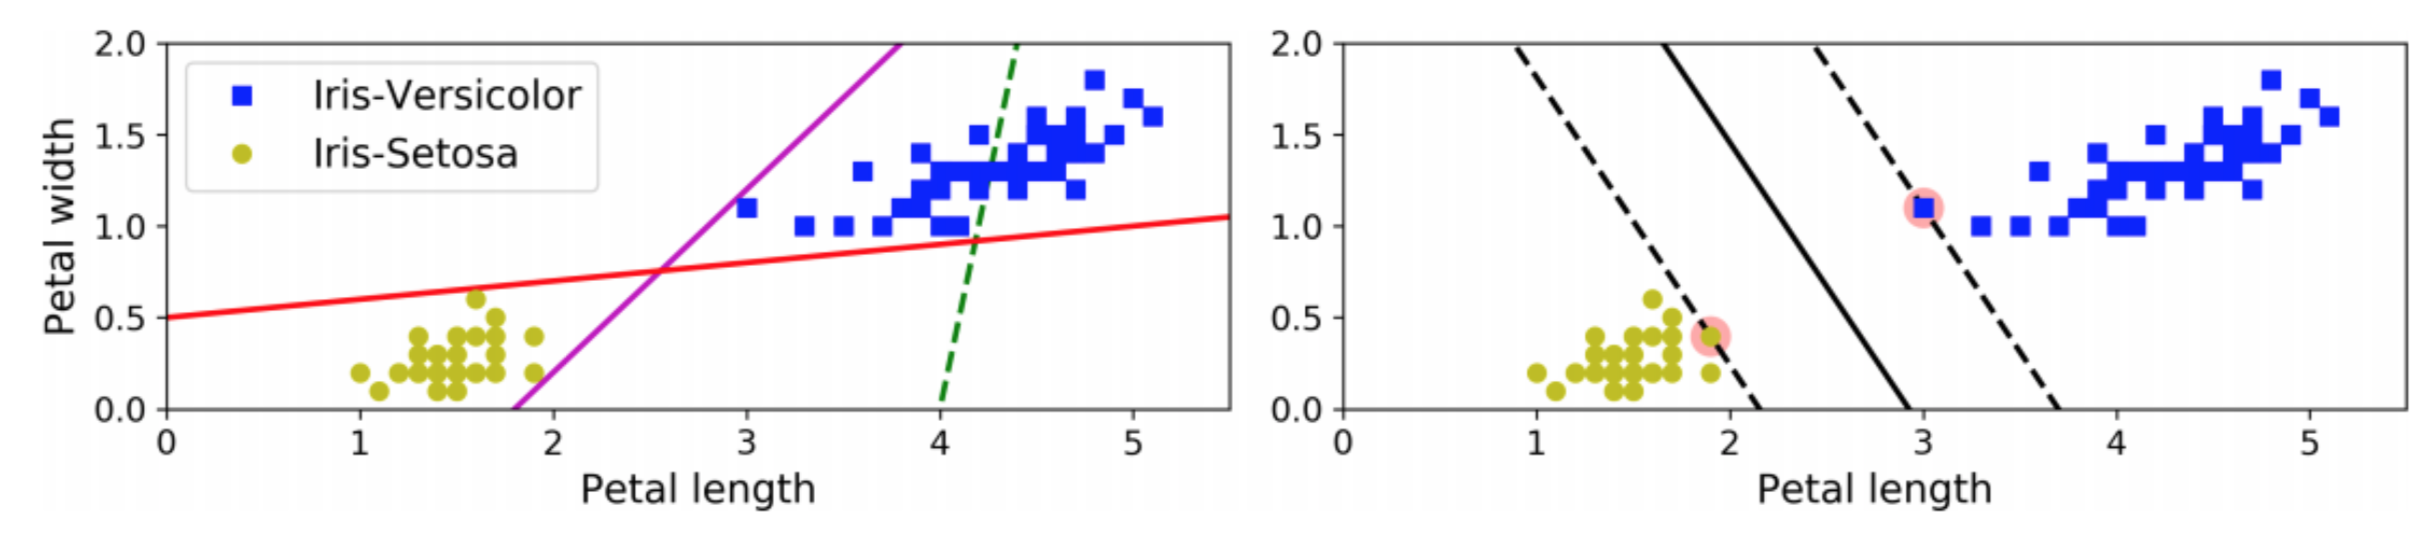
\includegraphics[scale = 0.35]{Pics/SVM}
	\caption{Example SVM}
\end{figure*}

\underline{Question} : What is the outcome of np.logspace(-8, 8, 17, base=2)? More generally, what is the outcome of np.logspace(-a, b, k, base=m)?\\


\underline{Answer} : The logspace function from the numpy package will return k numbers going from -a to b on a log scale with a log base m. 

\underline{Answer} : The outcome of np.logspace(-8, 8, 17, base=2) is a logarthmic space going from $2^{-8}$ to $2^8$ with 17 numbers equally spaced on log scale.
 The logspace function from the numpy package will return k numbers going from $m^{-a}$ to $m^b$ spaced on a log scale with a log base m. \\

\underline{Question} : What is the meaning of the warnings? What is the parameter responsible for its appearence? \\
 \underline{Answer} : The warning tells us that the algorithm did not converge, it did not reach the stop criterion. The parameter responsible for its appearence is the max_iter parameter. Its value is not sufficient for the algorithm to converge. The data variance is maybe too large for the algorithm to efficiently perform the SVM. \\

\underline{Question} : What did we change with respect to the previous run of LinearSVC()? \\
\underline{Answer}: We added a parameter MaxAbsScaler() to scale the absolute data between 0 and 1 and thus reduce the variance. \\

\underline{Question} : Explain what happens if we execute \\
\underline{Answer}: Those lines will execute a SVM with a maxabsscaler parameter but with no C parameter which is by default 1.0.\\

\underline{Question} : what is the difference between StandardScaler() and MaxAbsScaler()? What are other scaling options available in sklearn? \\
\underline{Answer}: StandardScaler will normalize the data : $\frac{x-m}{\sigma}$ with m the mean and $\sigma$ the standard deviation of data. It differs from StandarScaler because absolute values are mapped in the range [0,1]. \\

\underline{Question} : using the previous code as an example achieve test accuracy  ≥0.9 . You can use any method from sklearn package. Give a mathematical description of the selected method. Explain the range of considered hyperparamers.\\
\underline{Answer}: choose an algorithm and test


